\documentclass[11pt, oneside]{article} 	% use "amsart" instead of "article" for AMSLaTeX format
\usepackage{geometry} 		% See geometry.pdf to learn the layout options. There are lots.
\geometry{letterpaper}  		% ... or a4paper or a5paper or ... 
\usepackage[parfill]{parskip} 		% Activate to begin paragraphs with an empty line rather than an indent
\usepackage{graphicx}				% Use pdf, png, jpg, or eps§ with pdflatex; use eps in DVI mode
								% TeX will automatically convert eps --> pdf in pdflatex		
\usepackage{amssymb}
\usepackage{amsmath}
\usepackage{authblk}
\usepackage[
backend=biber,
style=alphabetic,
]{biblatex}
\usepackage{graphicx}
\graphicspath{ {./images/} }
\usepackage{verbatim}
\usepackage{tikz} 
\usepackage{subcaption}
\captionsetup{compatibility=false}



\usepackage{syntonly}

% \syntaxonly \langle -- use this for checking syntax only
% \mbox {text} - keep together
% \fbox {text} - keep together and draw around

%\pagestyle{plain|headings|empty} % header and footer p.27
%SetFonts
%\include{filename}, \includeonly{filename1, filename2} , \input[fiename}

%SetFonts% 


\title{Vandermone Determinants via Graph Tournaments}
\author{Dave Fetterman}
\affil{Obviously Unemployed}
\date{2/16/23}
\begin{document}
\maketitle

\begin{abstract}

In 2D space, two points $(x_1, y_1), (x_2, y_2), x_1 \neq x_2$ define a line, a polynomial of degree 1.  Three distinct points $(x_1, y_1), (x_2, y_2), (x_3, y_3), x_1 \neq x_2 \neq x_3$ define a parabola, a polynomial of degree 2.  In general, for finite univariate polynomials of nonnegative, whole degree, $n+1$ such points uniquely specify a polynomial of degree $n$.  Why?
\\

This is the farthest thing from a new result. This is a paper is instead a thoroughly awkward trip through a few mathematical domains including linear algebra and graph theory to arrive at this well known destination. Helicopters and cars both have their uses. But you wouldn't build a car by turning a helicopter on its side and adding wheels.  Metaphorically, I do, so you don't have to.

\end{abstract}

\section{Motivator: Polynomial Uniqueness in Interpolation}

If we have points $f(x_0) = y_0, f(x_1) = y_1,  \ldots f(x_{n}) = y_{n}$, how can we determine the coefficients $a_i$ of the polynomial $f(x) = a_0x^0 + a_1x^1 + \ldots + a_nx^n$?

This square matrix of width $n+1$, which I'll denote $X_n$, is known as a Vandermonde matrix\cite{1}, and models this set of $n+1$ equations as $X \cdot \vec{a} = \vec{y}$:

 $\begin{bmatrix}
1 & x_0 & x_0^2 & \ldots & x_0^{n} \\
1 & x_1 & x_1^2 & \ldots & x_1^{n} \\
\vdots & & & & \vdots  \\
1 & x_{n} & x_{n}^2 & \ldots & x_{n}^{n} \\
\end{bmatrix}
\cdot 
\begin{bmatrix}
a_0 \\
a_1 \\
\vdots \\
a_n \\
\end{bmatrix}
=
\begin{bmatrix}
y_0 \\
y_1 \\
\vdots \\
y_{n} \\
\end{bmatrix}
$
\\

Therefore, we can find our unique coefficient vector $\vec{a}$ if and only if we can solve $X_n \cdot \vec{a} = \vec{y}$, or $\vec{a} = X_n^{-1} \vec{y}$.  $\vec{a}$ has a unique solution if and only if $\det(X_n) \neq 0$.  
\\

\emph{The rest of this paper tries to find this determinant through a uniquely circuitous path.}

\section{Finding the Vandermonde determinant}

It should be noted that there are other, clearer methods of finding this determinant\cite{1} either starting with polynomial unqiueness (basically, going the ``other'' direction), abstract algebra, direct linear algebra, vector maps, and others.  These, however, were not the ones I stumbled on.

First, we know that for in any $X_n$, if any $x_i = x_j$ for distinct $i, j$, we have a zero determinant and no solution. If $f(x_i) = f(x_j)$ and $x_i = x_j$, then we are simply underdetermined (not enough points for a unique polynomial).   If $f(x_i) = f(x_j)$ and $x_i \neq x_j$, then we have an impossible vertical section of our graph.  Otherwise, we are in good shape to solve the above equation for $\vec{a}$.
\\

This suggests that every pair $(x_i, x_j), i < j$ corresponds to a factor  $(x_j - x_i)$ in the determinant, and that the determinant is then some multiple of $D = \prod_{0 \leq i < j \leq n}(x_j-x_i)$.

Taking $n=2$ as a base case ($n=1$ produces a boring constant $f(x)$), we see that 
 $\det\begin{bmatrix}
1 & x_0  \\
1 & x_1  \\
\end{bmatrix} = (x_1 - x_0)$, suggesting $D$ may be the determinant of a Vandermonde matrix.  
\\

Let's prove that it is.

\subsection{Setup: Vandermonde inductive step and main theorem}

\fbox{\textbf{Theorem}: The determinant of $X_n$ with generating coefficients $x_0, x_1 ... x_n$ is $\prod_{0 \leq i < j \leq n}(x_j-x_i)$.}

With the base case $n=1$ in hand, the rest of the paper handles the inductive step of proving the main theorem.  We assume in the inductive step that this determinant holds for Vandermonde matrices of size $n-1$ ($n-1$ generating coefficients, matrix with width $n$).

\textbf{Inductive Step of Proof of Theorem}:
\\

\fbox{If, for all $X_{n-1}$, $\det(X_{n-1}) = \prod_{0 \leq i < j \leq n-1}(x_j-x_i)$, then for all $X_{n}, \det(X_{n}) = \prod_{0 \leq i < j \leq n}(x_j-x_i)$}.

\subsubsection{Definitions} 

Let's create a few definitions: 
\begin{itemize}
\item Denote by $M_{k,n}$ the Vandermonde matrix  $X_n$ with column $n$ and row $k$ excluded\footnote{Note: I use zero-indexed matrices in this paper, since in the case of a Vandermonde matrix $X_n$, the zero-indexed entry $(i, j)$ neatly corresponds to $x_i^j$} , often called a ``matrix minor''.  
\item Given an ordered set of indices $I = [0, n]\in\mathbb{N}$, denote by $P_I$ the \emph{product} of all factors the form $(x_j - x_i)$, given $i < j$ and $i, j \in I$.  So $P_{[0,2]} = (x_1 - x_0)(x_2-x_0)(x_2- x_1)$.
\item Given an ordered set of indices $I = [0, n]\in\mathbb{N}$, denote by $S_I$ the \emph{sum} over all permutations\footnote{meaning, $\sigma \in Sym(I)$} $\sigma$  of $I$ of $sgn(\sigma) x_{\sigma(n)}^{n} x_{\sigma(n-1)}^{n-1} ... x_{\sigma(0)}^{0} $. So $S_{[0,2]} = x_2^2x_1^1x_0^0 - x_2^2x_0^1x_1^0 - x_1^2x_2^1x_0^0 + x_1^2x_0^1x_2^0 + x_0^2x_2^1x_1^0 - x_0^2x_1^1x_2^0$.
\end{itemize}

\subsubsection{Plan for Inductive Step of Vandermonde Derminant Proof} 

Using the definitions of $P_I, S_I$ from above, the main thrust of the paper is proving this algebraic statement:

\fbox{\textbf{The P-S Equivalence Lemma}: For a set of indices $I$, $P_I = S_I$.  }

This is the main statement we prove through the paper.

Assuming this is proven, the rest of the proof of the inductive step falls out quickly.  We'll get that out of the way.

\begin{itemize}
\item (1) $det(X_n) = \sum_{k=0}^n (-1)^{k+n} x_k^n\det(M_{k, n})$ 
\item (2) For our base base, $\det(\mathbf{X_1}) = P_{[0,1]}$
\item (3) By inductive hypothesis $det(M_{k,n}) = \sum_{k=0}^n (-1)^{k+n} x_k^n P_{[0,n] - \{k\}}$
\item (4) $\sum_{k=0}^n (-1)^{k+n}  x_k^n S_{[0,n] -\{k\}} = S_{[0, n]}$
\item (5) By the Lemma, (4) means $\sum_{k=0}^n (-1)^{k+n}  x_k^n P_{[0,n] -\{k\}} = P_{[0, n]}$
\item (6) Therefore, transitively, $det(X_n) = P_{[0, n]} = \prod_{0 \leq i < j \leq n}(x_j-x_i)$.
\end{itemize}

\subsubsection{Straightforward Steps (1)-(6) in Plan}

(1) is the minor-based definition of the determinant.

The determinant of 
 $X = \begin{bmatrix}
1 & x_0 & x_0^2 & \ldots & x_0^{n} \\
1 & x_1 & x_1^2 & \ldots & x_1^{n} \\
\vdots & & & & \vdots  \\
1 & x_{n} & x_{n}^2 & \ldots & x_{n}^{n} \\
\end{bmatrix}
$ can be calculated down the rightmost column as

$\det(X) = (-1)^n [ x_0^n \det(M_{0,n}) - x_1^n \det(M_{1,n}) +  ... + (-1)^n x^n \det(M_{n,n})]$.
\\

(2) is clear, with 
$\det(\begin{bmatrix} 1 & x_0 \\ 1& x_1 \end{bmatrix})$
$= -1\cdot(1\cdot M_{1, 1} - 1 \cdot M_{0,1}) = $
$(x_1 - x_0) = P_{[0,1]}$.

(3) says inductively, we can presuppose that  for any $M_{k, n}$, \emph{which is itself a Vandermonde matrix of smaller size}, $\det(M_{k,n})$ can be expressed as $P_{[0,n] - \{k\}}$

(4) This simply partitions all terms of the form $sgn(\sigma) x_{\sigma(n)}^{n} x_{\sigma(n-1)}^{n-1} ... x_{\sigma(0)}^{0}$, $\sigma \in Sym(I)$ into those that start with $x_k^n$ and no $x_k$ in the tail, summed over all $k$.   On  $I = \{c,b,a\}$, for example, the terms split out exactly into $c^2(b^1a^0 - b^0a^1) - b^2(c^1a^0-a^1c^0) + a^2(c^1b^0-b^1c^0) = c^2b^1a^0 - c^2a^0b^1 - b^2c^1a^0 + b^2a^1c^0 + a^2c^1b^0 - a^2b^1c^0$.

(5) follows from applying the $P$-$S$ equivalence Lemma to swap instances of $S$ with those of $P$ in (4).

(6) Following the equalities all the way back to 1, $\det(X_n)$ is then $P[0,n]$.

\section{Proof of $P_{[0,n]} = S_{[0,n]}$}

First, let's establish some algebraic intuition with an example.

\subsection{Example: $P{[0,1]} = S{[0,1]} \Rightarrow P{[0,2]} = S{[0,2]}$}
We've already established that $P_{[0,1]} = (x_1 - x_0) =  x_1^1x_0^0 - x_0^1x_1^0 = S_{[0,1]}$.  To see that $P_{[0,2]} = S_{[0,2]}$, write it out:

\begin{align}
P_{[0,2]}  \\
= (x_2-x_1)(x_2-x_0)P_{[0,1]} \\
= (x_2-x_1)(x_2-x_0)S_{[0,1]} \\
= x_2^2(x_1^1x_0^0 - x_0^1x_1^0) \\
+ x_2x_0(x_1^1x_0^0 - x_0^1x_1^0) \\
- x_2x_1 (x_1^1x_0^0 - x_0^1x_1^0) \\
+ x_1x_2(x_1^1x_0^0 - x_0^1x_1^0)  \\
= x_2^2x_1^1x_0^0  + x_1^2x_0^1x_2^0 + x_0^2x_2^1x_1^0   \\
 - x_2^2x_0^1x_1^0 - x_1^2x_2^1x_0^0 - x_0^2x_1^1x_2^0 \\
+ x_0^1x_1^1x_2^1 - x_0^1x_1^1x_2^1 \\
= S_{[0,2]}
\end{align}

Note that line (3) follows from line (2) by base case, line (8) is the set of even permutations of $\{2,1,0\}$, line (9) the odds, and line (10) becomes zero by combining terms with the same exponents and opposite signs (or opposite $sgn(\sigma)$, if you like).

\subsection{Graph Intuition}

In the general case, the difficulty is really line (10) - how do we do all the cancellations?

Rather than handle these $2^{\begin{pmatrix}n\\2\end{pmatrix}}$ terms by hand each time algebraically, through an isomorphism, we'll translate these factors $(x_j - x_i)$ as a set of $\begin{pmatrix} n\\2\end{pmatrix}$ \emph{graphs}.

The $2^{\begin{pmatrix}n\\2\end{pmatrix}} = 2^{\begin{pmatrix}3\\2\end{pmatrix}} = 8$ terms expanded on lines (8) - (10) are clearly the 8 terms resulting from multiplication of the three factors $(x_2 - x_1)(x_2-x_0)(x_1-x_0)$.  Each such algebraic term is isomorphic to one of the complete\footnote{edges between every vertex} directed\footnote{an edge points toward one of its vertices} graphs (also known as ``tournaments'') in the set on 3 nodes, with the edge ``pointing'' from the selected term towards the omitted term in $(x_j - x_i)$.

For example, the term $x_2^2x_1^1x_0$, produced by multiplying the three left terms of the three factors of $(x_2-x_1)(x_2-x_0)(x_1-x_0)$, corresponds to graph 1a.  

\begin{figure}
\centering
\begin{subfigure}{.5\textwidth}
  \centering
  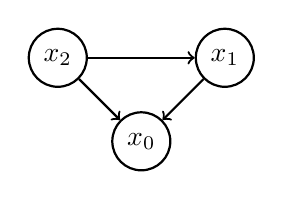
\begin{tikzpicture}[node distance={15mm}, thick, main/.style = {draw, circle}] 
\node[main] (1) {$x_0$}; 
\node[main] (2) [above right of=1] {$x_1$}; 
\node[main] (3) [above left of=1] {$x_2$}; 
\draw[->] (3) -- (2); 
\draw[->] (3) -- (1);
\draw[->] (2) -- (1);
\end{tikzpicture}
  \caption{($\mathbf{x_2}-x_1)(\mathbf{x_2}-x_0)(\mathbf{x_1}-x_0) \rightarrow x_2^2x_1^1x_0^0$}
  \label{fig:sub1}
\end{subfigure}

\begin{subfigure}{.5\textwidth}
  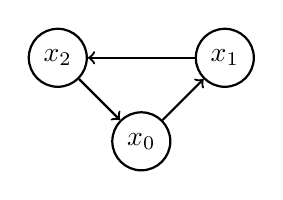
\begin{tikzpicture}[node distance={15mm}, thick, main/.style = {draw, circle}] 
\node[main] (1) {$x_0$}; 
\node[main] (2) [above right of=1] {$x_1$}; 
\node[main] (3) [above left of=1] {$x_2$}; 
\draw[<-] (3) -- (2); 
\draw[->] (3) -- (1);
\draw[<-] (2) -- (1);
\end{tikzpicture}

  \caption{($x_2-\mathbf{x_1})(\mathbf{x_2}-x_0)(x_1-\mathbf{x_0}) \rightarrow x_2^1x_1^1x_0^1$}
  \label{fig:sub2}
\end{subfigure}

\begin{subfigure}{.5\textwidth}
  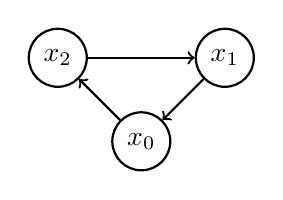
\begin{tikzpicture}[node distance={15mm}, thick, main/.style = {draw, circle}] 
\node[main] (1) {$x_0$}; 
\node[main] (2) [above right of=1] {$x_1$}; 
\node[main] (3) [above left of=1] {$x_2$}; 
\draw[->] (3) -- (2); 
\draw[<-] (3) -- (1);
\draw[->] (2) -- (1);
\end{tikzpicture}

  \caption{($\mathbf{x_2}-x_1)(x_2-\mathbf{x_0})(\mathbf{x_1}-x_0) \rightarrow -x_2^1x_1^1x_0^1$}
  \label{fig:sub3}
\end{subfigure}


\caption{Three terms of  $P_{[0,2]}$, corresponding to complete directed graphs of size 3}
\label{fig:test}
\end{figure}

The term $x_2^1x_1^1x_0^1$, from multiplying the right, left, and right terms of the above product corresponds to 1b.  And, in 1c, the inverted product sequence left, right, left, produces the inverted graph cycle and notably, the algebraic inverse $-x_2^1x_1^1x_0^1$ in the product expansion (sum).

This should give a flavor of the proof: \emph{To find the expansion of $P_I$ and show it equals $S_I$, we show each of the $2^{\begin{pmatrix}n \\ 2\end{pmatrix}}$ graphs produced when expanding $P_I$ are isomorphic to a term in the sum like $-x_1^2x_2^1x_0^0$, where each exponent represents the ``out degree'' of a vertex $x_i$ in the graph. If any of the exponents in the term corresponding to a graph are equal, we show the term drops out in the final cancellation, and through the same isomoprhism, we are left with $S_I$.}

\subsection{P-S Equivalence Lemma Proof layout}

Here is a layout of the proof that $P_I=S_I$.

First, we prove a set of lemmas:
\begin{itemize}
\item (1) Lemma: There is an isomorphism between the set of terms in an expanded $P_{[0,n]} =\prod_{0 \leq i < j \leq n}(x_j - x_i)$ and the set of all possible tournaments of size $n+1$.
\item (2) Lemma: All tournaments are either acyclic or contain a 3-cycle.
\item (3) Lemma: Acyclic tournaments correspond through the isomorphism with terms of the form $sgn(\sigma) x_{\sigma(n)}^nx_{\sigma(n-1)}^{n-1}  ... x_{\sigma(0)}^{0}$ for some permutation $\sigma$ on $[0,n]$.
\item (4) Lemma: Cyclic tournaments with a 3-cycle can be paired 1:1 with an otherwise identical graph with that 3-cycle inverted.
\end{itemize}

Through these lemmas, we can start with a base case equality $P_{[0,2]} = S_{[0,2]}$ and show:
\begin{itemize}
\item The isomorphism equates the set of edge configurations in of adding an additional node $x_n$ to an acyclic graph $G$ of $n$ nodes with the algebraic action of multiplying $\prod_{0 \leq i \leq n-1}(x_n-x_i)$ by $P_{[0,n-1]}$. 
\item (6) This isomorphism maps all possibilities of adding an additional node $x_n$ to an acyclic graph $G$ of $n$ nodes to $S_{[0,n]}$.  In particular, all terms corresponding to graphs with cycles cancel, and only those corresponding to acyclic tournaments remain in the sum.   
\item (7) Because $P_{[0,n]}$ and $S_{[0,n]}$ map to the same set of graphs \emph{through the same bijection (isomorphism)}, this shows the \textbf{P-S equivalency lemma}, and the inductive step of the Vandermonde Determinant Proof.
\end{itemize}

\subsection{Lemma 1}

\emph{There is an isomorphism between the set of terms in an expanded $P_{[0,n]} =\prod_{0 \leq i < j \leq n}(x_j - x_i)$ and the set of all possible tournaments of size $n+1$.}

Every possible complete directed graph  $G = (E,V)$ of vertex size $n$  consists exactly of edges $(i, j)$\footnote{of some direction} with $i, j \in [v_0, v_n-1], i < j$.  If $(i \rightarrow j) \in E$, then consider $(\mathbf{x_i} - x_j)$ in the expansion of $P_{[0, n-1]}$; otherwise if $(j \rightarrow i) \in E$, then consider $(x_i - \mathbf{x_j})$ in the expansion of $P_{[0, n-1]}$.  Conversely, if $(\mathbf{x_i} - x_j)$ is in a term of $P_{[0, n-1]}$, take $(i \rightarrow j)$ for an edge in the graph, otherwise $(j \rightarrow i)$.  As in Figure 1, this isomorphism should be straightforward.
\footnote{Or consider pulling out $Q = P_{[0,n]}/(x_i - x_j)$.  Then $(x_i - x_j)Q = x_iQ - x_jQ$, two graph sets with different ``selections'' for edge $(i,j)$}

\emph{Note: We call this bijective correspondence between an algebraic term in the expansion of $P_{[0,n]}$ and a tournament on $n+1$ nodes ``the isomorphism'' throughout the paper. When we say a graph ``pairs with an algebraic form'' or a algebraic term ``has a corresponding graph'', it's meant to be through this bijection.}

\subsection{Lemma 2}

\emph{All directed complete graphs are either acyclic or contain a 3-cycle.}

If the graph contains no cycles, or a cycle of length 3, we are done.

If a graph contains some cycle through vertices $(v_0 \rightarrow v_{1} \rightarrow  ...  \rightarrow v_{m-1} \rightarrow  v_0)$ of length $m > 3$, we can split it into two possible cycles: $A = (v_0 \rightarrow  v_{1} \rightarrow v_{2} \leadsto  v_0)$ and $B = (v_{2} \rightarrow  v_{3} \rightarrow  ... \rightarrow v_{0} \leadsto v_{2} )$, with $\leadsto$ meaning ``maybe goes to''.  Depending on the direction of edge $(v_{0}, v_{2})$, exactly one of $A$ or $B$ must be a cycle.  If $A$ is a cycle, we are done.  Else use $B$ and reapply recursively on this smaller cycle, eventually down to a cycle of length 3.

\subsection{Lemma 3}

\emph{Acyclic tournaments correspond through the isomorphism with terms of the form $sgn(\sigma) x_{\sigma(n)}^nx_{\sigma(n-1)}^{n-1}  ... x_{\sigma(0)}^{0}$ for some permutation $\sigma$ on $[0,n]$.}


Another way of saying ``every acyclic tournament maps through some $\sigma$ to$sgn(\sigma) x_{\sigma(n)}^nx_{\sigma(n-1)}^{n-1}  ... x_{\sigma(0)}^{0}$ is ``No acyclic tournament has nodes of equal outdegree''.  For example, an acyclic tournament on a set of nodes indexed $[0, 3]$ necessarily looks like the following:

\begin{figure}
  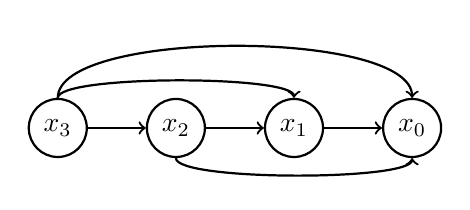
\begin{tikzpicture}[node distance={15mm}, thick, main/.style = {draw, circle}] 
\node[main] (4) {$x_3$}; 
\node[main] (3) [right of=4] {$x_2$}; 
\node[main] (2) [right of=3] {$x_1$}; 
\node[main] (1) [right of=2] {$x_0$}; 
\draw[->] (4) -- (3); 
\draw[->] (4) to [out = 90, in = 90, looseness=.25] (2);
\draw[->] (4) to [out = 90, in = 90, looseness=.5] (1);
\draw[->] (3) to [out = 270, in = 270, looseness=.25] (1);
\draw[->] (3) -- (2);
\draw[->] (2) -- (1);
\end{tikzpicture}
\caption{An acyclic tournament on 4 nodes}
\label{fig:test2}
\end{figure}


Every vertex here $x_i$ has a unique outdegree $k \in [0,n-1]$, which, through the isomorphism, we see as the exponent of $x_i$ in the graph's algebraic form.  The above graph corresponds to the term $x_3^3x_2^2x_1^1x_0^0$.  As every edge here ``points right'', it's clear that there can be no cycle (or particularly, 3-cycle).

For the converse, consider the statement that ``no acyclic tournament has a subgraph\footnote{Meaning a copy of the original graph with some vertices and all their adjacent edges removed} with two or more vertices of equal degree''.  If this is true then certainly the graph has to have the above form out outdegrees.  To see this:

\begin{itemize}
\item If the graph is of the form $sgn(\sigma) x_{\sigma(n)}^nx_{\sigma(n-1)}^{n-1}  ... x_{\sigma(0)}^{0}$ for some $n$ and some $\sigma$, we are done.
\item Suppose then it has two vertices with duplicate outdegrees, but has no cycles. Eliminate vertices, starting from $x_n$, then $x_{n-1}$, down to $x_2$ just until a subgraph is of the form with all unique outdegrees, which we'll call\footnote{Note: the set of $y$ are the same as the set of $x$, just with some other indexing} $y_{m} ... y_0$ with $y_m$ of outdegree $m$ and $y_0$ of outdegree 0.  Call $y_0$ for now $y^-$.
\item Add the last removed vertex $y^*$ and its edges back.  $y^*$ must have the same outdegree as some other vertex, otherwise we have a contradiction.
\item Step: If $(y^- \rightarrow y^*)$ is in the graph, then necessarily there is a cycle $(y^- \rightarrow y^* \rightarrow $ some $y_j \rightarrow y^-)$, so we have a contradiction.
\item Else $(y^* \rightarrow y^-)$ is in the graph, so the outdegree of $y^*$ can't be 0.  Remove $y^-$, reducing all vertices by outdegree 1, creating a new $y^- \neq y^*$ with minimum degree, and go back to (Step).
\end{itemize}

From this, we can conclude that an acylic directed tournament has vertices of all unique degrees, and thus, up to vertex labeling (permutation), has the algebraic form $sgn(\sigma) x_{\sigma(n)}^nx_{\sigma(n-1)}^{n-1}  ... x_{\sigma(0)}^{0}$  for some $\sigma$.

\subsection{Lemma 4}

\emph{Cyclic tournaments with a 3-cycle can be uniquely paired 1:1 with an otherwise identical graph with that 3-cycle inverted.}

\begin{figure}
\centering
\begin{subfigure}{.9\textwidth}
  \centering
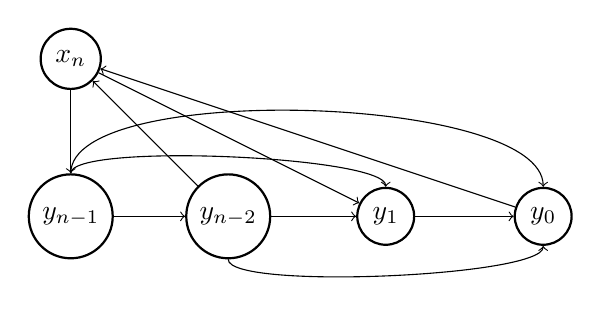
\begin{tikzpicture}
\begin{scope}[every node/.style={circle,thick,draw}]
    \node (5) at (0,2) {$x_n$};
    \node (4) at (0,0) {$y_{n-1}$};
    \node (3) at (2,0) {$y_{n-2}$};
    \node (2) at (4,0) {$y_1$};
    \node (1) at (6,0) {$y_0$};
\end{scope}

\draw[->] (4) -- (3); 
\draw[->] (4) to [out = 90, in = 90, looseness=.25] (2);
\draw[->] (4) to [out = 90, in = 90, looseness=.5] (1);
\draw[->] (3) to [out = 270, in = 270, looseness=.25] (1);
\draw[->] (3) -- (2);
\draw[->] (2) -- (1);
\draw[->] (5) -- (4); 
\draw[<-] (5) -- (3); 
\draw[->] (5) -- (2); 
\draw[<-] (5) -- (1); 
\end{tikzpicture}
  \caption{G: $x_n^2y_{n-1}^3y_{n-2}^3y_{1}^1y_0^1$}  
  \label{fig:sub1}
\end{subfigure}
\begin{subfigure}{.9\textwidth}
  \centering
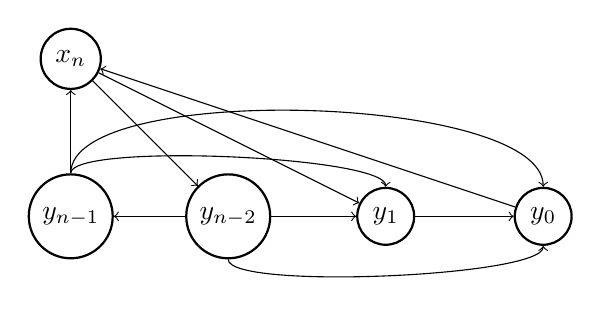
\begin{tikzpicture}
\begin{scope}[every node/.style={circle,thick,draw}]
    \node (5) at (0,2) {$x_n$};
    \node (4) at (0,0) {$y_{n-1}$};
    \node (3) at (2,0) {$y_{n-2}$};
    \node (2) at (4,0) {$y_1$};
    \node (1) at (6,0) {$y_0$};
\end{scope}

\draw[<-] (4) -- (3); 
\draw[->] (4) to [out = 90, in = 90, looseness=.25] (2);
\draw[->] (4) to [out = 90, in = 90, looseness=.5] (1);
\draw[->] (3) to [out = 270, in = 270, looseness=.25] (1);
\draw[->] (3) -- (2);
\draw[->] (2) -- (1);
\draw[<-] (5) -- (4); 
\draw[->] (5) -- (3); 
\draw[->] (5) -- (2); 
\draw[<-] (5) -- (1); 
\end{tikzpicture}
  \caption{G: $-x_n^2y_{n-1}^3y_{n-2}^3y_{1}^1y_0^1$}  
  \label{fig:sub2}
\end{subfigure}
\caption{Adding $x_n$ can turn acyclic tournaments into cyclical ones}
\label{fig:test3}
\end{figure}


Suppose, for a graph $G$ we fix an ordering of vertices like $\{x_n, x_{n-1}, x_{n-2}... x_0\}$.  Suppose $(x_a, x_b, x_c)$ is the 3-cycle with highest lexicographic order of the vertex set ($x_n > x_{n-1} > ...$), with edges pointing either direction.  Then, the graph $G'$, with the same edges, except the direction of cycle  $(x_a, x_b, x_c)$ reversed:
\begin{itemize}
\item (1) Can be mapped to uniquely to G, and vice versa.
\item (2) Has an algebraic representation through the main bijection which is an inverse to that of G.
\end{itemize}

(1) is clear because each uniquely determines the other; the order of vertices is the same, thus the ``first'' cycle is the same, and the order need only be reversed.  In Figure 3, the ``first'' cycle would be $(x_n, y_{n-1}, y_{n-2})$, even though the graph has many other cycles.
\\
(2) Reversing $(\mathbf{x_1} - x_2)(\mathbf{x_2}-x_3)(\mathbf{x_3}-x_1) = x_1x_2x_3$ yields $(x_1 - \mathbf{x_2})(x_2-\mathbf{x_3})(x_3-\mathbf{x_1}) = -x_1x_2x_3$, for any choice of $x_1, x_2, x_3$.  \footnote{Note that in 3b, the graph without $x_n$ is still a tournament by Lemma 3, as its algebraic representation has  gone from $y_{n-1}^3y_{n-2}^2y_{1}^1y_0^0$ to $-y_{n-2}^3y_{n-1}^2y_{1}^1y_0^0$ with the reversal of edge $(y_{n-1}, y_{n-2})$.}


\subsection{Step 5}

\begin{figure}
\centering
\begin{subfigure}{.9\textwidth}
  \centering
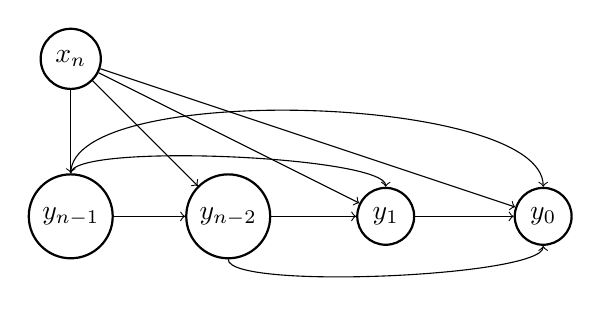
\begin{tikzpicture}
\begin{scope}[every node/.style={circle,thick,draw}]
    \node (5) at (0,2) {$x_n$};
    \node (4) at (0,0) {$y_{n-1}$};
    \node (3) at (2,0) {$y_{n-2}$};
    \node (2) at (4,0) {$y_1$};
    \node (1) at (6,0) {$y_0$};
\end{scope}

\draw[->] (4) -- (3); 
\draw[->] (4) to [out = 90, in = 90, looseness=.25] (2);
\draw[->] (4) to [out = 90, in = 90, looseness=.5] (1);
\draw[->] (3) to [out = 270, in = 270, looseness=.25] (1);
\draw[->] (3) -- (2);
\draw[->] (2) -- (1);
\draw[->] (5) -- (4); 
\draw[->] (5) -- (3); 
\draw[->] (5) -- (2); 
\draw[->] (5) -- (1); 
\end{tikzpicture}
  \caption{G: adding $x_n$ to a tournament of 4 nodes $\simeq x^4y_{n-1}^3y_{n-2}^2y_{1}^1y_0^0$}  \label{fig:sub1}
\end{subfigure}
\begin{subfigure}{.9\textwidth}
  \centering
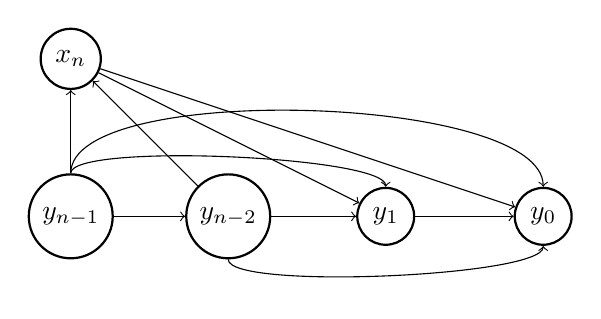
\begin{tikzpicture}
\begin{scope}[every node/.style={circle,thick,draw}]
    \node (5) at (0,2) {$x_n$};
    \node (4) at (0,0) {$y_{n-1}$};
    \node (3) at (2,0) {$y_{n-2}$};
    \node (2) at (4,0) {$y_1$};
    \node (1) at (6,0) {$y_0$};
\end{scope}

\draw[->] (4) -- (3); 
\draw[->] (4) to [out = 90, in = 90, looseness=.25] (2);
\draw[->] (4) to [out = 90, in = 90, looseness=.5] (1);
\draw[->] (3) to [out = 270, in = 270, looseness=.25] (1);
\draw[->] (3) -- (2);
\draw[->] (2) -- (1);
\draw[<-] (5) -- (4); 
\draw[<-] (5) -- (3); 
\draw[->] (5) -- (2); 
\draw[->] (5) -- (1); 
\end{tikzpicture}
  \caption{G: adding $x_n$ to a tournament of 4 nodes:  $\simeq y_{n-2}^4y_{n-1}^3x^2y_{1}^1y_0^0$}
  \label{fig:sub1}
\end{subfigure}
\caption{Adding $x_n$ to an existing tournament on 4 nodes}
\label{fig:test3}
\end{figure}


\emph{The isomorphism equates the set of edge configurations in of adding an additional node $x_n$ to an acyclic graph $G$ of $n$ nodes with the algebraic action of multiplying $\prod_{0 \leq i \leq n-1}(x_n-x_i)$ by $P_{[0,n-1]}$. }

By inductive assumption, suppose an acyclic tournament graph $G = (E, V)$ on a permutation of the vertices $y_{n-1}, y_{n-2}, ... y_0 \in V$ is constructed such that $(y_i \rightarrow y_j) \in E$ iff $i > j$.

Then, let's add a new vertex $x_n$ to the tournament, which necessarily has connections to all of $\{y_{n-1}...y_0\}$ (Figure 4a).


Each of the $2^n$ terms (before any cancellation) resulting from $\prod_{0 \leq i < n}(x_n-x_i)$ correspond 1:1 with one of the $2^n$ settings of the edges from $x_n$ to every other $x_i$.  These are coupled with the expressions $P_{[0,n]}$ and the graph on vertices $x_0, .... x_{n-1}$, respectively.

The above graph would correspond to the term $(\mathbf{x_n}-y_{n-1})(\mathbf{x_n}-y_{n-2})(\mathbf{x_n}-y_{1})(\mathbf{x_n}-y_{0})P_{[0,n-1]}$ in $S_{[0,n]}$.


\subsection{Step 6}

\emph{This bijection maps all possibilities of adding an additional node $x_n$ to an acyclic graph $G$ of $n$ nodes to $S_{[0,n]}$.}

Looking at Figures 3a and 3b, notice that, when adding $x_n$, if at any point there are edges $(x_n \rightarrow y_{j}), (y_{i} \rightarrow x_n), i < j$, then we necessarily have a cycle in the graph.  By Lemma 4, these each are mapped 1:1 to another graph, which has an inverted ``first cycle'' and is an algebraic inverse.  Thus, each pair of these contributes $0$ to an expanded $P_{[0,n]}$.

So the only configurations of $x_n$'s edges that do not create a cycle are those that point ``out'' from $x_n$ and then shift permanently to pointing ``in'' to $x_n$ as we descend from $y_{n-1}, y_{n-2} ... y_0$, like Figures 4a and 4b. By Lemma 3, in the algebraic representation these correspond exactly to $sgn(\sigma) y_{n-1}^{n}y_{n-2}^{n-1}...y_{k}^{k+1}x_n^ky_{k-2}^{k-1}...y_0^0$. 

Notice that the sum, over all permutations $\sigma \in Sym([0,n])$, is exactly $S_{[0,n]}$. 


\subsection{Step 7: Wrapping up}

We assumed $P_{[0, n-1]} = S_{[0, n-1]}$.

Expanding $P_{[0,n]}$ algebraically is difficult.  Instead, we mapped it through the graph-algebraic isomorphism to a set of graphs.  Separating cyclic and acyclic graphs, we saw, through the same isomorphism back, that cyclic graphs cancel on the algebraic side, and acyclic graphs remained, leaving the sum of every permutation of  
\\
$sgn(\sigma) x_{\sigma(n)}^{n} x_{\sigma(n-1)}^{n-1} x_{\sigma(n-2)}^{n-2} ... x_{\sigma(0)}^{0}, \sigma \in Sym([0,n])$.

This is $S_{[0,n]}$.

Having proved the \textbf{The P-S Equivalence Lemma}, we finish the inductive step of the Vandermonde Determinant Proof (chapter 2).

\section{Example of adding $x$ to a tournament of 4 nodes} 

Algebraically resolving $P_{[0,n]} = \prod_{0 \leq i, j, \leq n, j < j} (x_i - x_j)$ gets increasingly unwieldy to show, so we'll conclude with an example of adding all possibilities of $x$ with directed edges to a single existing acyclic tournament\footnote{When doing handwork like this, using $a,b,c$ feels more natural than $x_0, x_1, x_2...$}  with order $d > c > b > a$, with representation $d^3c^2b^1a^0$.
\\

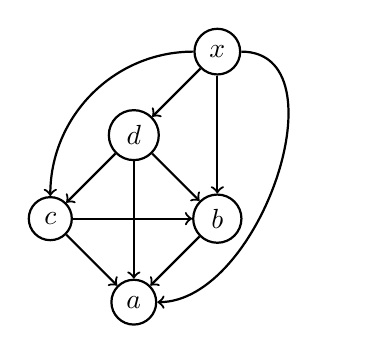
\begin{tikzpicture}[node distance={15mm}, thick, main/.style = {draw, circle}] 
\node[main] (1) {$a$}; 
\node[main] (2) [above right of=1] {$b$}; 
\node[main] (3) [above left of=1] {$c$}; 
\node[main] (4) [above right of=3] {$d$}; 
\node[main] (5) [above right of=4] {$x$}; 
\draw[->] (5) -- (4);
\draw[->] (5) to [out=180, in=90, looseness=1] (3); 
\draw[->] (5) -- (2);
\draw[->] (5) to [out=0, in=0, looseness=1] (1); 
\draw[->] (4) -- (3); 
\draw[->] (4) -- (2); 
\draw[->] (4) -- (1); 
\draw[->] (3) -- (2); 
\draw[->] (3) -- (1);
\draw[->] (2) -- (1);
\end{tikzpicture}
\\

The tournament represented by $q=x^4d^3c^2b^1a^0$

The chart maps all $2^4$ terms $t$ in $p=(x-a)(x-b)(x-c)(x-d)$ multiplied by existing tournament representation $q=d^3c^2b^1a^0$, with the ``product'' $t \cdot q$ representing one of the $2^4$ possible 5-node graphs.

These products either:
\begin{itemize}
\item Are isomorphic to an acyclic graph, so are of the form $sgn(\sigma)  \sigma(x)^{4} \sigma(d)^{3} \sigma(c)^{2} \sigma(b)^{1} \sigma(a)^0$
\item Are isomorphic to a graph with a cycle in $\{(x, d, c), (x,c,b), (x,b,a)\}$.  If so, they have a uniquely matching pair $t^*$ and graph $q^*$ when flipping their first cycle.
\end{itemize}



\begin{center}
\begin{tabular}{||c c c c||} 
 \hline
t & $t \cdot q$ & Matching factor $t^*$ $\cdot$ Matching $q^*$ & First cycle \\ [0.5ex] 
 \hline\hline
 $x^4$ & $x^4d^3c^2b^1a^0$ none & none \\ 
 \hline
 $-x^3a$ & $-x^3d^3c^2b^1a^1$ & $-x^3b \cdot -d^3c^2a^1b^0$ & $(x,b,a)$ \\ 
 \hline
 $-x^3b$ & $-x^3d^3c^2b^2a^0$ & $-x^3c \cdot -d^3b^2c^1a^0$ & $(x,c,b)$ \\ 
 \hline
 $-x^3c$ & $-x^3d^3c^3b^1a^0$ & $-x^3d \cdot -c^3d^2b^1a^0$ & $(x,d,c)$ \\ 
 \hline
 $-x^3d$ & $-x^3d^4c^2b^1a^0$ & none & none \\ 
 \hline
 $x^2ba$ & $x^2d^3c^2b^2a^1$ & $x^2ca \cdot -d^3b^2c^1a^0$ &  $(x,c,b)$ \\ 
  \hline
 $x^2ca$ & $x^2d^3c^3b^1a^1$ & $x^2da  \cdot -c^3d^2b^1a^0$ &  $(x,d,c)$ \\ 
 \hline
 $x^2da$ & $x^2d^4c^2b^1a^1$ & $x^2db  \cdot -d^3c^2a^1b^0$ &  $(x,b,a)$ \\ 

 \hline
 $x^2cb$ & $x^2d^3c^3b^2a^0$ & $x^2db  \cdot -c^3d^2b^1a^0$ &  $(x,d,c)$ \\ 
 \hline
 $x^2db$ & $x^2d^4c^2b^2a^0$ & $x^2dc  \cdot -d^3b^2c^1a^0$ &  $(x,d,c)$ \\ 
 
 
\hline
 $x^2dc$ & $x^2d^4c^3b^1a^0$ & none &   none \\ 
 
 \hline
 $-xcba$ & $-xd^3c^3b^2a^1$ & $-xdba  \cdot -c^3d^2b^1a^0$ &  $(x,d,c)$ \\ 

 \hline
 $-xdba$ & $-xd^4c^2b^2a^1$ & $-xcba  \cdot -d^3b^2c^1a^0$ &  $x,c,b)$ \\ 

 \hline
 $-xdca$ & $-xd^4c^3b^1a^1$ & $-xdcb  \cdot -d^3c^2a^1b^0$ &  $(x,b,a)$ \\ 

 \hline
 $-xdcb$ & $-xd^4c^3b^2a^0$ & none &  none \\ 
 
 
 \hline
 $dcba$ & $ d^4c^3b^2a^1 $ & none &  none \\ 
 
 \hline
\end{tabular}
\end{center}

This sum, $x^4d^3c^2b^1a^0-x^3d^4c^2b^1a^0+x^2d^4c^3b^1a^0-xd^4c^3b^2a^0+d^4c^3b^2a^1$, when added to the tables of all the other initial settings of $q$, produces $S_{[0,4]}$.


\begin{thebibliography}{9}
\bibitem{1}
Wikipedia: \url{https://en.wikipedia.org/wiki/Vandermonde_matrix}
\end{thebibliography}


\end{document}

